%%%------------------------------------------------------------------------------%%%
%%% Seiteneinstellungen %%%
%%%------------------------------------------------------------------------------%%%

\documentclass[12pt,oneside,a4paper]{scrreprt}
\usepackage[left=3.5cm,right=2.5cm,top=2.5cm,bottom=2.5cm,includeheadfoot]{geometry}	
\usepackage{silence}
\WarningFilter{scrbook}{Usage of package `fancyhdr'}	
\usepackage{scrhack}
\usepackage{epigraph}
\usepackage{xcolor}
\usepackage{genealogytree}


%%%------------------------------------------------------------------------------%%%
%%% benötigte Pakete %%%
%%%------------------------------------------------------------------------------%%%

\linespread{1.25}\selectfont
\usepackage{fancyhdr} % Für die Kopf- und Fußzeilen
\usepackage{graphicx} 
\usepackage{float} 
\usepackage{paralist} %Für Liste mit Pfeilen 
\usepackage{graphics} % Zum Einbinden von Bildern mit \includegraphics
\usepackage[british,UKenglish,USenglish,english,american]{babel}
\usepackage[utf8]{inputenc}
\usepackage{textcomp} % Umlaute
\usepackage[numbers,round]{natbib} 
%\usepackage{natbib} % Literaturverweise mit (Autor Jahr) nach DIN
\definecolor{links}{HTML}{2A1B81}
\usepackage[unicode=true, pdfusetitle,bookmarks=true,bookmarksnumbered=true,bookmarksopen=true, breaklinks=false,pdfborder={0 0 1},backref=section,colorlinks, linkcolor = black, citecolor = black, filecolor = black, urlcolor = links]{hyperref}

\usepackage{url}
\usepackage{listings}
%\usepackage{picins} --> veraltet

% disable footnotes numbering reset in each chapter
\usepackage{remreset}
\makeatletter
\@removefromreset{footnote}{chapter}
\makeatother

\setlength{\headheight}{1.1\baselineskip}

%%%------------------------------------------------------------------------------%%%
%%% Variablen %%%
%%%------------------------------------------------------------------------------%%%

\newcommand{\Seitenbreite}{155mm}
\newcommand{\Seitentexthoehe}{230mm}
\newcommand{\SeitentexthoeheHALB}{115mm}
\newcommand{\MYtitle}{Entw. einer JEE Web-Anwendung}
\newcommand{\MYauthor}{Marcel Mittelstädt}
\newcommand{\MYdate}{02. September 2011}
\newcommand{\mycomment}[1]{}

%%%------------------------------------------------------------------------------%%%
%%% Ränder, Absatzabstände etc. %%%
%%%------------------------------------------------------------------------------%%%

\setlength{\parskip}{1ex plus0.5ex minus0.2ex} % Absatzabstand etwas größer
\setlength{\itemsep}{0ex plus0.2ex} % Abstand zweier Listenelemente kleiner
\parindent=0cm % Kein Absatzeinzug
\parskip=1mm % Abstand zwischen 2 Absätzen

%%%------------------------------------------------------------------------------%%%
%%% Abkürzungsverzeichnis, Glossar und Listings strukturieren %%%
%%%------------------------------------------------------------------------------%%%

\usepackage{nomencl}
\let\abk\nomenclature
\renewcommand{\nomname}{List Of Abbreviations}
\setlength{\nomlabelwidth}{.20\hsize}
\renewcommand{\nomlabel}[1]{#1 \dotfill}
\setlength{\nomitemsep}{-\parsep}
\makenomenclature
% makeindex hauptdatei.nlo -s nomencl.ist -o hauptdatei.nls erst Latex dan Konsole dann Latex

\renewcommand\lstlistingname{Code Snippet}
\renewcommand\lstlistlistingname{List Of Code Snippets}
\def\lstlistingautorefname{Ausz.}

%%%------------------------------------------------------------------------------%%%
%%% Formatierung von Quellcodes %%%
%%%------------------------------------------------------------------------------%%%

\usepackage{xcolor} % Text farbig markieren 
\usepackage{calc}
\definecolor{lightgrey}{HTML}{F5F5F5}
\definecolor{lightgreen}{HTML}{669900}
\definecolor{colKeyWords}{HTML}{A52A33}
\definecolor{colComments}{HTML}{0733FF}
\definecolor{colIdentifiers}{HTML}{371D42}

\lstset{%
float=hbp,%
language=Java, %
basicstyle=\ttfamily\small, %
identifierstyle=\color{colIdentifiers}, %
keywordstyle=\color{colKeyWords}\textbf, %
stringstyle=\color{colComments}, %
commentstyle=\color{lightgreen}, %
columns=flexible, %
tabsize=2, %
frame=single, %
extendedchars=true, %
showspaces=false, %
showstringspaces=false, %
numbers=left, %
numberstyle=\tiny, %
breaklines=true, %
backgroundcolor=\color{lightgrey}, %
breakautoindent=true, %
captionpos=b%
} 

%%%------------------------------------------------------------------------------%%%
%%% Kopf- und Fußzeileneinstellungen %%%
%%%------------------------------------------------------------------------------%%%

\pagestyle{fancy}
\fancyhf{}


	\renewcommand{\headrulewidth}{0.5pt}
	
	\pagenumbering{Roman}
	\fancyfoot[L]{\today}
	\fancyfoot[R]{\thepage}
	\renewcommand{\footrulewidth}{0.5pt}



%%%------------------------------------------------------------------------------%%%
%%% Jetzt geht die Arbeit richtig los: %%%
%%%------------------------------------------------------------------------------%%%
\usepackage{nameref}
\begin{document}
%%%------------------------------------------------------------------------------%%%
%%% Die Titelseite und Vorwort %%%
%%%------------------------------------------------------------------------------%%%
\begin{titlepage} 
\thispagestyle{empty} % Keine Kopf- und Fusszeilen

\begin{center}
\Huge{\textbf{BIG DATA}}\\[1.0 cm]

\Large{An Introduction To The Fields Of Data Engineering, Development And Architecture Of Data-Intensive Applications.}\\[2.0 cm]

\Large{\textemdash Winter Semester 2018 \textemdash}\\[0.5 cm]
\large{Munich, \today}\\[5.3 cm]

\line(1,0){380}\\[0.6 cm]

\normalsize{\textbf{Marcel Mittelstädt}}\\
Mail: \href{mailto:mittelstaedtmarcel@googlemail.com}{mittelstaedtmarcel@googlemail.com}\\
Web: \href{http://www.marcel-mittelstaedt.com}{www.marcel-mittelstaedt.com}\\[0.8 cm]

\textbf{Cooperative State University Baden-Wuerttemberg}\\

\includegraphics[width=0.3\textwidth]{dhbw_logo.png}\\

\end{center}

\end{titlepage}
%%%------------------------------------------------------------------------------%%%
%%% Die Verzeichnisse %%%
%%%------------------------------------------------------------------------------%%%

\newpage
%%%------------------------------------------------------------------------------%%%
%%% Preface %%% 
%%%------------------------------------------------------------------------------%%%

\underline{\textbf{\LARGE{Preface}}}\\[2cm]
This lecture will give you a brief introduction to so what is called 'Big Data'. We will quickly refresh the basics about databases, data models and data processing you have learned so far and compare those to the distributed world of Big Data. \\
After that we will take a deep dive into the foundations of distributed data storages and data processing as well as the belonging concepts of reliability, scalability, replication, partitioning, batch and stream processing. \\
Later on we will take a look at the most common used software and frameworks (mostly the hadoop ecosystem). \\
At the end, as you know the basic concepts and you are able to setup and work with distributed environments and huge data sets, there will be a short introduction to data science. \\

At the end of each lesson, there will be some hands-on exercises, which we will start together and which have to be finished till the next week.
This lecture will only be about 36 hours in 12 weeks (1 slot each week), which is very little time to cover such an extensive topic. So pay close attention and if you can't keep up, feel free to ask questions at the end of each lesson. \\

You can find:
\begin{samepage}
\begin{itemize}
	\item this \textbf{script} (and \LaTeX{}-sources),
	\item \textbf{slides} presented within the lecture,
	\item \textbf{excercises} and \textbf{solutions},
	\item \textbf{docker images}, \textbf{scripts} as well as \textbf{sample data sets}
\end{itemize}
\end{samepage}
here:
\begin{lstlisting}[language=bash,frame=none,numbers=none,xleftmargin=0.05\textwidth,xrightmargin=0.05\textwidth]
 https://github.com/marcelmittelstaedt/BigData
\end{lstlisting}

You can just download everything directly or install \lstinline{git} and get everything by using:
\begin{lstlisting}[language=bash,frame=none,numbers=none,xleftmargin=0.05\textwidth,xrightmargin=0.05\textwidth]
 git clone https://github.com/marcelmittelstaedt/BigData.git
\end{lstlisting}
and 
\begin{lstlisting}[language=bash,frame=none,numbers=none,xleftmargin=0.05\textwidth,xrightmargin=0.05\textwidth]
 git pull
\end{lstlisting}
to get the most recent version.\\

If you find any mistakes or misspellings feel free to send me a mail\\
(\textbf{\href{mailto:mittelstaedtmarcel@googlemail.com}{mittelstaedtmarcel@googlemail.com}})
or if you are able to, commit a push request.\\

One last point, as you may have noticed, Microsoft as well as other commercial vendors successfully fail at developing and providing adequate solutions for highly data-driven applications, so almost any software or framework you will encouter during this lecture or later, will be open-source and only be runnable on a UNIX-based operating system. Either you are already familiar with UNIX (lucky you), otherwise you will learn something valuable that will improve your life.\\

\setlength{\epigraphwidth}{0.9\textwidth}
\setlength\epigraphrule{0pt}
\epigraph{\itshape ``Microsoft is not the answer. Microsoft is the question. NO is the answer.''}{--- Erik Naggum \gtrsymDied~, \textit{Philantropist and Developer (Emacs, Lisp and SGML) }}



\setcounter{tocdepth}{2}
\tableofcontents % Inhaltsverzeichnis


%%%---------------------------------------------------------------------------------------%%%
%%% An dieser Stelle sollen die eingebundenen Kapitel %%%
%%% erscheinen, dafür die vorhin angelegten Kapitel entfernen %%%
%%%---------------------------------------------------------------------------------------%%%

\pagenumbering{arabic}
\setcounter{table}{1}
\setcounter{secnumdepth}{3}
\pagestyle{fancy}
\fancypagestyle{plainn}
{
	\fancyhead[R]{%
	% We want italics
	%\itshape
	% The chapter number only if it's greater than 0
 	%\chaptermark
	% The chapter title
	\leftmark}
	\renewcommand{\headrulewidth}{0.5pt}
	
	\fancyfoot[L]{\MYdate}
	\fancyfoot[R]{\thepage}
	\renewcommand{\footrulewidth}{0.5pt}
}	% Extracommand damit die Header und Footer um ToC richtig sind
\pagestyle{plainn}
\abk{DHBW}{Duale Hochschule Baden-WŸrttemberg}


\nocite{w3}
 %blinde Zitate, Quellenverweise, Abkürzungen etc.

\chapter{Introduction To Big Data}
\label{chapter_bigdata}
\setlength{\epigraphwidth}{0.95\textwidth}
\setlength\epigraphrule{0pt}
\epigraph{\itshape ``Big Data is like teenage sex: everyone talks about it, nobody really knows how to do it, everyone thinks everyone else is doing it, so everyone claims they are doing it.''}{--- Dan Ariely, \textit{Professor of Psychology and Behavioral Economics,\\ Duke University}}


Lorem Ipsum

\begin{figure}[ht]
	\centering
  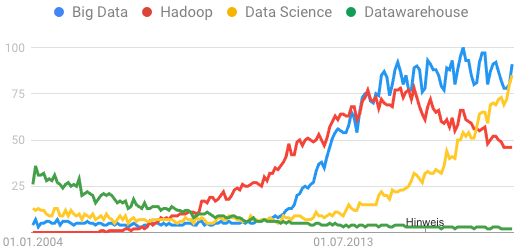
\includegraphics[width=1.0\textwidth]{google_trends_bigdata.png}
	\caption{Schema - Google Trends (Popularity Of Certain Search Terms)}
	\label{google_trends_bigdata}
\end{figure}


\section{Distributed Computing}
\label{bd_hwe}

CPU RAM Vertical to horizontal Scalability --> Distributed Computing
Data volume increases
Data processing increases
Scale out vs Up
Cloud provider 
- Lets rent a super computer
Cloud vs Custer Computing
Containerization
MapR IaaS, PaaS, SaaS


to-be-added

\newpage
\section{BigData V's}
\label{bd_vs}
Firstly introduced by Gartner in 2011\footnote{\cite{GRTNRVS}, https://www.gartner.com/newsroom/id/1731916} the (initial) \textit{3 V's of Big Data} quickly became key characteristics and challenges of Big Data. Back in this time the focus on Big Data was on the volume of data alone, ignoring the \textit{variety} of information (databases, documents, video, social media) and \textit{velocity} of information (how fast it is being produced and how fast it needs to be processed) as well. \\
Today some more V's have established (Figure \ref{bigdata_vs}), we will quickly disscuss them within the next chapters.

\begin{figure}[ht]
	\centering
  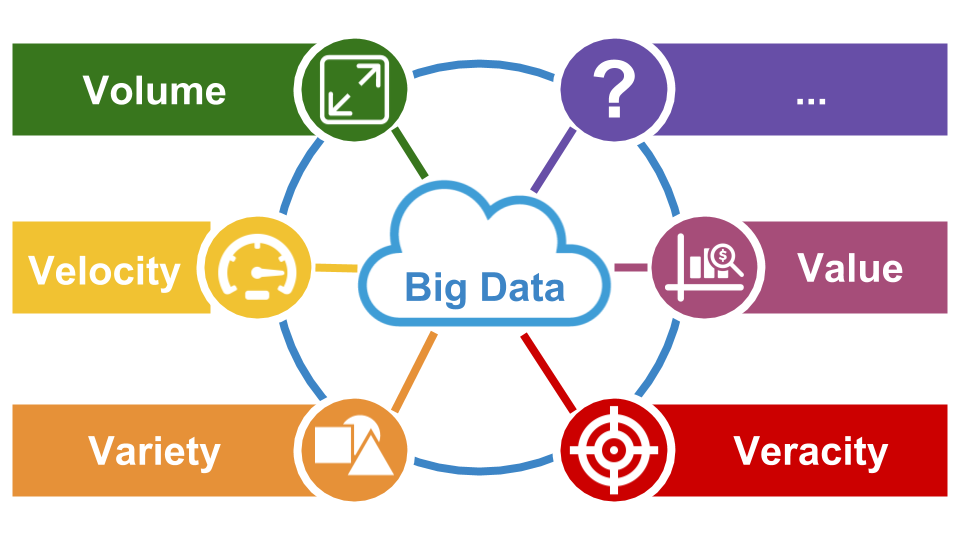
\includegraphics[width=0.8\textwidth]{bigdata_vs.png}
	\caption{Schema - Big Data V's}
	\label{bigdata_vs}
\end{figure}

\subsection{Volume}
\label{bd_vs_volume}
\textit{Volume} sounds quiet obvious as we are talking about Big Data, but what is Big in terms of volume? Let's have a quick look at some examples: 
\begin{itemize}
	\item \textbf{Wikipedia:} in 2014 the english part of Wikipedia as well as Wikipedia Commons (including Media like Images, Videos etc.) had a size of around 23TB\footnote{\cite{WPS}, https://en.wikipedia.org/wiki/Wikipedia:Size\_of\_Wikipedia}.
	\item \textbf{Spotify:} in 2013 data generated by users of was about 1,5TB per day which approximately means 534TB per year\footnote{\cite{SPTFYV}, https://de.slideshare.net/AdamKawa/big-data-at-spotify}.
	\item \textbf{Google:} the search index currently has a size of 100PB\footnote{\cite{GSIS}, https://www.google.com/search/howsearchworks/crawling-indexing/}.\\
\end{itemize}

But Big Data does not need to be about those kind of sizes. As a rule of thumb, data that can easily be handled (e.g. processed, saved or queried) within a traditional database (e.g. PostgreSQL, Informix, DB2, Oracle etc.) and belonging datawarehouse, like a few gigabytes per week or month, is not Big Data. \\
But it's not unlikely that there is an adequate Big Data case in your immediate surrounding, for instance if you are running a mid-level e-commerce shop and make use of tracking data like web server log files (e.g. produced by Apache, Nginx) or data provided by third-party tracking tools like Google Analytics or WebTrekk with the aim to analyze the behaviour of visitors of your website, you easily end up with several terabytes of logfiles/tracking data per year, which needs to be processed. If you would like to calculate cohorts or a CLV\abk{CLV}{Customer Lifetime Value}\footnote{\textit{CLV - Customer Lifetime Value, prediction model which calculates the net profit attributed to the entire future relationship with a customer based on the past}} this would even require processing the data of several years and in this way probably more than 10TB of data at once.


\subsection{Velocity}
\label{bd_vs_velocity}
\textit{Velocity} in terms of Big Data has two facets: how fast data is produced and how fast it needs to be processed to be able to make use of or react to it. Depending on the use case it is required to react within minutes or even seconds. Let's have a quick look at some examples: 

\begin{itemize}
	\item \textbf{Facebook:} in 2012 every 60 seconds 510.000 comments, 293.000 status updates and 136.000 photos had been posted on average, which needed to be processed in near real-time\footnote{\cite{TSSFP}, http://thesocialskinny.com/100-social-media-statistics-for-2012/}.
	\item \textbf{Twitter:} in 2013 usually 500 million tweets were posted each day on Twitter, which means 5.7000 Tweets per second on average\footnote{\cite{TWTTPS}, https://blog.twitter.com/engineering/en\_us/a/2013/new-tweets-per-second-record-and-how.html}.
	\item \textbf{Google:} According to Internet Live Stats, Google is handling around 6 billion search requests per day, which approximately means 70.000 per second.\footnote{\cite{ILSGS}, http://www.internetlivestats.com/google-search-statistics/}.\\
\end{itemize}

But your data-system does not need to handle those kind of velocities to be called BigData. For instance if your working for mid-level bank like ING Netherlands, you need to handle 1 million transactions per day, which is ``just'' 12 requests per second. But those requests need to be handled in real-time. Additionally during the processing of those requests (transactions) several data science models need to be involved and executed to be able to detect fraudulent transactions as they happen, to protect the bank and its customers. ING Netherland achieves this by using Apache Kafka\footnote{\cite{KAFKAHP}, https://kafka.apache.org/} for queuing events and streaming them into Apache Flink\footnote{\cite{FLINKHP}, https://flink.apache.org/} to apply machine learning models\footnote{\cite{DAING}, https://data-artisans.com/blog/real-time-fraud-detection-ing-bank-apache-flink}. \\
Real-time data processing and running data science models on it, is not just a case for the big players like Facebook, Twitter and Google, for instance fraud detection on transactions is also quiet interesting if your company runs a mid-level e-commerce shop or if it is an insurance company as well. If you run a website and want to customize the content in real-time, so that a visitor sees what he would like to see (based on his previous behaviour on the website) you probably end up with \textit{onsite-personalization} which also requires real-time data processing and applying data-science models. \\
This is just a glimpse of characteristics, challanges and possible use cases in terms of data \textit{velocity} and Big Data.

\subsection{Variety}
\label{bd_vs_variety}
\textit{Variety} refers to the diversity of data sources, so called ``Big Data'' data-systems need to handle. Those data sources and their structures are widely diversified and cannot easily be handled by traditional relational databases. Let's have a look at a few examples and put them into 3 well known categories: \textit{structured data}, \textit{semi-structured data} and \textit{utructured data}.\\


\begin{itemize}
	\item \textbf{Structured Data:} means plain data structures which have fixed attributes/columns, specific data types and a defined domain. Related but different kinds of data records can easily be linked using constraints of the relational data model, like primary and foreign keys. This kind of data can easily (almost directly) be stored into a traditional SQL database or similar.\\
	\item \textbf{Semi-Structured Data:} covers all data structures, that do not easily fit into the constraints of the relational data model and in this way into a relational SQL database. Even though semi-structured data has of course some organizational properties that makes it easy to categorize, link and analyze the data. With ``some'' additional work it is possible to store this kind of data in a relational SQL database, but as this will violate many constraints of the relational data model, you would end up making a lot of compromises, e.g. in terms of defined domains, expected structures, or extensibility which do not fit very well into the relational world or only with a lot of operational overhead and workarounds. Semi-structured data has some structure in terms of tags and attributes but those and nested structures as well will usually change from document to document or data record to record. The semi-structured data model has some serious advantages: no need to worry about \textit{object-relational impedance mismatch} and support for highly nested and hierarchical data and in this way simplified data models but it is also more prone to \textit{``grabage-in, garbage-out''} as important constraints of the relational model are thrown away. Examples of semi-structured data are:
	\begin{itemize}
		\item \textbf{JSON} documents (e.g. provided by the Facebook Graph API\footnote{\cite{FBGAPI}, https://developers.facebook.com/docs/graph-api/using-graph-api/} or the Twitter API\footnote{\cite{TWTAPI}, https://developer.twitter.com/en/docs/tweets/data-dictionary/overview/tweet-object.html}), 
		\item \textbf{XML} documents (e.g. provided by the Google Maps Geocoding API\footnote{\cite{GMGCAPI}, https://developers.google.com/maps/documentation/geocoding/intro} or the OpenWeatherMap Weather API\footnote{\cite{OWMAPI}, https://openweathermap.org/api}) or
		\item \textbf{HTML} documents, for instance if your developing a web crawler (e.g. using Scrapy\footnote{\cite{SCPYHP}, https://scrapy.org/} for data gathering or Selenium\footnote{\cite{SELEHP}, https://www.seleniumhq.org/} for testing purposes).\\
	\end{itemize}
	\item \textbf{Unstructured Data:} is everything that is neither structured or semi-structured. This usually includes:
	\begin{itemize}
		\item \textbf{Natural language}, for instance Social Media Posts (e.g. Facebook and Twitter), Ratings (e.g. on Amazon, IMDB or other platforms) or plain text (e.g. Wikipedia articles, product information on Amazon or any e-commerce shop) you may want to analyze by \textit{natural language processing} with the purpose of calculating a sentiment (\textit{What do customers think about your product?}) or the meaning and truthfulness of a rating (\textit{Is the review positive or negative? Is it fake?}). 
		\item \textbf{Geographical data}, for instance satellite, GPS, radar or sonar data and images with the purpose of analyzing meteorological, vecicular or seismic behaviour, e.g. for the purpose of predicting the future.
		\item \textbf{Photos and Videos}, for instance of traffic and surveillance cameras to analyze and optimize traffic flow or for the sake of security.
		\item \textbf{Scientific data}, like physic measuring and sensor data, seismic imagery or athmospheric data to analyze and optimize a physics experiment. For instance CERN makes use of Hadoop for unstructured sensor data, to unlock insights from machine data\footnote{\cite{CERNH}, https://conferences.oreilly.com/strata/stratany2014/public/schedule/detail/36312}
		\end{itemize}
\end{itemize}

\subsection{Veracity}
\label{bd_vs_veracity}
Speaking about Big Data, \textit{veracity} is about the trustworthiness and accuracy of a certain dataset. Especially in terms of accuracy it is not just about the quality of the data itself, but also tasks of quality assurance and data cleansing, like removing bias, superfluous, redundant or just duplicate records or attributes. Trustworthiness is also highly vulnerable to the volatility of the data (which you usually cannot control), as a lot of data sources and related records frequently change in their lifetime. For instance an account balance quickly changes over time (due to ongoing transactions) as well as people which have liked a topic, post or site on a social media platform may dislike it the next day. Additionaly there are a lot more possible mistakes, caused by humans or machines, like wrong system timestamps, an incomplete or corrupted dataset may causing a complete different result. Even if you have a fully-fletched environment which ensures data quality in its own limits, you cannot be sure the data you are processing is 100\% accurate, as their could already be a mistake in the source system. For instance if you are processing data from a tracking system and you are able to ensure 100\% completeness of data and accuracy within your ETL processes (e.g. using automated tests like FitNesse\footnote{\cite{FITNHP}, http://docs.fitnesse.org/FrontPage}), their could already be a significant bias in the source system, as a related tracking pixel may not have been properly configured on every page of your e-commerce shop (e.g. due to a relaunch of your website), so you are maybe missing some page views and products viewed in your tracking data. Or much simpler, an issue that even the tracking sytsem cannot handle: people who disable third party cookies, they will always appear as new visitors in your tracking data, even if its the 10th time they visit your e-commerce shop. \\
As analytics and related conclusions rely on the quality of the data, a Big Data data-system should always try to achieve the best data quality possible, even it is seen a lot: \textit{Garbage In - Garbage Out} is not acceptable.


\subsection{Value}
\label{bd_vs_value}
Last but probably most important of all V's is the \textit{value}. We previously discussed \textit{volume}, \textit{velocity}, \textit{variety} and \textit{veracity} - all of them are meaningless if you dont derive business \textit{value} from your data, but they are also significant enabler and success factors for the \textit{value} of your data. We will quickly discuss the correlation now: 
\begin{itemize}
	\item \textbf{Volume:} the more data you collect, the more insights you can probably gather and the more informed your insights and decisions may be. But its not only about the volume, if your company does not have the ressources and capabilities to perform the required analysises on collected data and perform the derived actions, \textit{volume} is menaingless.
	\item \textbf{Velocity:} Today everything is about speed, especially business. The faster data is collected and available for analysis processes, the faster it can be used for decision-making processes.
	\item \textbf{Variety:} The more data sources you connect to your data-system, the more insights you can potentially create and probably you will no longer rely an a single data source for a certain business object (like a client), which overall increases data quality and depth. Enabling you, for instance to build customer journeys, calculate a CLV, and in this way improve engagement and retention. At the end the \textit{value} of your data increases.
	\item \textbf{Veracity:} This is quiet obvious, as the more trustworthy and accurate your data is, more business critical desicisions and applications will rely on it and in this way the revenue of your company will probably increase as well as the value of your data.\\ 
\end{itemize}

\textit{Value} can probably be found in any kind of data, but the challenge is to pick the right data and use it the right way. First of all you need to understand the potential, benefits and have an idea of what you want to achieve. For instance use it to understand your customers better, (re-)target them accordingly in advertisements or increase engagement by onsite-personalization and recommendation engines. Maybe you want to optimize processes or machine and ressource utilization or just analyze log files to identify security violations or netwerk performance issues. There is an infinite number of cases a Big Data data-system can create business value. \\
If you just do not want to throw data away, there are cheaper and more appropriate solutions than a Big Data data-system. 

\subsection{Other V's}
\label{bd_vs_other_vs}
to-be-added

\section{Challenges}
\label{bd_def}
to-be-added

\section{BigData Use Cases}
\label{bd_def}
to-be-added

\section{BigData And Consistency}
\label{bd_consistency}
to-be-added

ACID
CAP
BASE

\section{BigData in Business}
\label{bd_bdib}
to-be-added

\subsection{Roles}
\label{bd_bdib_roles}
to-be-added

Roles
- Data Engineer
- Data Scientist
- Ops

\subsection{BI vs DataScience}
\label{bd_bdib_bi_vs_datascience}
to-be-added


\subsection{Dissociation Datawarehousing}
\label{bd_bdib_diss_dwh}
to-be-added

\section{Definition of Big Data}
\label{bd_def}
to-be-added
\\[0.5 cm]
\hspace*{4mm}%
\fbox{%
  \hspace*{1.5mm}\hspace*{-1\fboxsep}%
  \parbox{0.08\textwidth + 5mm - 2\fboxsep}{%
\begin{minipage}{0.1\textwidth}

\includegraphics[width=\linewidth]{gear_brain.png}
\end{minipage}
  }%
}\hspace*{4mm}%
\begin{minipage}{0.8\textwidth}\raggedright
\textbf{BigData} is a term for data sets that are so large or complex that traditional database management tools or data processing software is inadequate to deal with them. \\
\end{minipage}\\[0.4 cm]

\section{Big Data Science}
\label{bd_science}
to-be-added
\chapter{Fundamentals Of Distributed Data Systems}
\label{chapter_technical_foundation}
\setlength{\epigraphwidth}{0.95\textwidth}
\setlength\epigraphrule{0pt}
\epigraph{\itshape ``I'm not telling you it's going to be easy - I'm telling you it's going to be worth it.''}{--- Arthur L. Williams Jr., \textit{Founder of Primerica Financial Services}}

In this chapter we will go trough the foundation of data systems, requirements and concepts which apply to any (data-driven) system. This covers in particular following topics:
\begin{samepage}
\begin{itemize}
	\item Section \ref{tf_nfreq} Requirements of \textbf{\nameref{tf_nfreq}}, e.g. 
		\begin{itemize}
			\item \ref{tf_nfreq_scalability} \nameref{tf_nfreq_scalability}, 
			\item \ref{tf_nfreq_avrel} \nameref{tf_nfreq_avrel}, 
			\item \ref{tf_nfreq_maintainability} \nameref{tf_nfreq_maintainability}.
		\end{itemize}
	\item Section \ref{tf_storageconcepts} \textbf{\nameref{tf_storageconcepts}} for databases
	\item Section \ref{tf_dma} \textbf{\nameref{tf_dma}} concepts
	\item Section \ref{tf_dds} \textbf{\nameref{tf_dds}}, e.g.
		\begin{itemize}
			\item \ref{tf_dds_partitioning} \nameref{tf_dds_partitioning}, 
			\item \ref{tf_dds_replication} \nameref{tf_dds_replication}, 
			\item \ref{tf_dds_transactions} \nameref{tf_dds_transactions}, 
			\item \ref{tf_dds_consistency} \nameref{tf_dds_consistency} amongst others.\\
		\end{itemize}
\end{itemize}
\end{samepage}

At the end you will have a basic understanding about the difference between common and distributed systems and databases, the basic concepts of each of them and which one theoretically fits best to solve a certain problem.
A more hands-on deep-dive into related software, frameworks as well as specific problems and use cases will be demonstrated later in chapter \ref{chapter_software_frameworks} \nameref{chapter_software_frameworks}.

\section{Data-Driven Systems}
\label{tf_nfreq}
When we think about data-driven systems, we mostly think about the same requirements we expect of any other data system we already know:
\begin{itemize}
	\item \textbf{Data Storage}: We need to store data and also need to be able to find it again later (\textit{database}). 
	\item \textbf{Data Querying}: We need to be able to query and filter data efficiently in certain kinds of ways (\textit{transaction and indices}).
	\item \textbf{Retention and Performance}: We want results fast, especially of expensive read operations (\textit{caching}).
	\item \textbf{Data Processsing}: We want to be able to process a huge amount of data (\textit{batch processing}) as well as process data asynchronously (\textit{stream processing}).\\
\end{itemize}

This sounds quite obvious, but remember those requirements are still the same as for the first database CODASYL\footnote{https://en.wikipedia.org/wiki/CODASYL} back in the 1960's. Even though there are and have been a lot of databases back in time, each of them with a diverse purpose and different approaches to solve e.g. indexing or caching - all of them still match those same requirements. Certainly those data systems evolved much further, especially within the last years, you may noticed:
\begin{itemize}
	\item Relational Databases being able to handle NoSQL data (e.g. even ``retirees'' like IBM DB2\footnote{\cite{IBMDB2JS}, https://www.ibm.com/support/knowledgecenter/en/SSEPEK\_11.0.0/json/src/tpc\\/db2z\_jsonfunctions.html} or Oracle\footnote{\cite{ORCLJS}, https://docs.oracle.com/database/121/ADXDB/json.htm}) as well as NoSQL databases being able to handle traditional SQL (e.g. ToroDB\footnote{\cite{TORODB}, https://www.torodb.com}) or
	\item databases becoming message queues (e.g. RethinkDB\footnote{\cite{RDBMQ}, https://rethinkdb.com/docs/changefeeds/} or Redis\footnote{\cite{RUDMQ}, https://redis.io/commands/rpoplpush}\footnote{\cite{BSARN}, see 5. Adopting Redis for Application Data}) and the other way around message queueing systems become databases (e.g. Apache Kafka\footnote{\cite{KFKQU}, https://kafka.apache.org/10/documentation/streams/developer-guide/interactive-queries.html}).\\
\end{itemize}

As you can see, boundaries between traditional databases and data-driven applications get blurred and in the same way more diversified. 
There is no one-size-fits-all solution, e.g. like you can find back in the past in the 1990's or early 2000s. 
At that time monolithic single-, 2 and 3-tier, architectures were state-of-the-art (see Figure \ref{schema_application_architectures} left-hand side). \\
Usually the \textbf{database layer} was represented by a data store like MySQL, Oracle, DB2 or even just files containing data stored on the local disk.\\
The \textbf{application layer} was usually a monolithic application developed in languages like PHP, Perl, C++ or Java and running on a web- or application server (e.g. Apache HTTP Server or IBM WebSphere).\\
And last but not least the \textbf{client layer}: a web browser like nowadays.\\
\begin{figure}[ht]
	\centering
  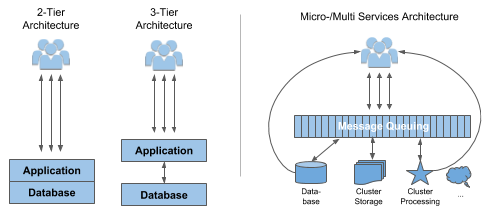
\includegraphics[width=1\textwidth]{application_architectures.png}
	\caption{Schema - Application Architectures}
	\label{schema_application_architectures}
\end{figure}
If you take a look at Figure \ref{schema_ebay_architecture_1997_1999} on page \pageref{schema_ebay_architecture_1997_1999} you can see an example of this time you may know: ebay.com. They have used the classical 3-tier architecture as well: Oracle as the database running on Solaris as OS\footnote{OS, Operating System}\abk{OS}{Operating System}, C++ as application code running on the Microsoft IIS\footnote{\cite{IIS}, \textit{Microsoft Internet Information Services, an extensible web server created by Microsoft for use with the Windows NT family.}} web server.
\begin{figure}[ht]
	\centering
  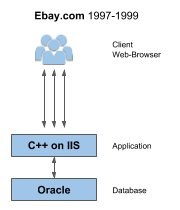
\includegraphics[width=0.4\textwidth]{ebay_architecture_199799.png}
	\caption{Schema - Architecture Ebay.com 1997-1999}
	\label{schema_ebay_architecture_1997_1999}
\end{figure}
As you can already guess, this architecture won't scale very well today, in fact the only way to scale this application was to upgrade the single server (\textit{scale up vertically}), in case of ebay.com they once switched from commodity hardware to a very pricey mainframe server (Sun Enterprise E10000\footnote{\cite{EBAYA}, slide 11}) to buy some time. But as you may have noticed there are much more ovious issues, e.g. if you think about:
\begin{itemize}
	\item \textbf{Redundancy} does not exist at all (if the database itself or it's server suffers an outage the whole system will be unavailable.
	\item \textbf{Extensability} is not existent, the system is only able to scale up vertically and if this is needed, a downtime is inevitable, as no part of the data system is neither replicated nor virtualized.
	\item \textbf{Maintainablity} is also very limited as any maintenance of the database will require a certain amount of time in which the application will be unavailable.
\end{itemize}
But we will dicuss this later in the following chapters.\\

The previously mentioned issues are already sufficient reason but also the increasing amount of data as well as required features of data systems these days (becoming more diversified in the same way) make it unfeasible to rely on a single tool. Instead each functionality is usually broken down into parts which can be done efficiently by suitable tools which are sticked together within the applications itself. This could probably look like as you can see in Figure \ref{schema_application_architectures} (right-hand side) on page \pageref{schema_application_architectures}, but that's just one plain example of many other.\\

Instead of having one single-purpose data store, there are several tied together, each one of them to fulfill it's specific part within the whole data system but all of them tied together as one application. \\
As you can see one part of the data system could be: a \textbf{database} (like you saw in Figure \ref{schema_ebay_architecture_1997_1999} on page \pageref{schema_ebay_architecture_1997_1999}), e.g. to store and serve:\\
\begin{itemize}
	\item user data (e.g. in case of an application with login)
	\item product data (e.g. in case the applications is a web shop)
	\item user generated content  (e.g. in case the application is a newspage, blog or forum)\\
\end{itemize}
Another part could be \textbf{cluster storage} like Hadoop, which could:\\
\begin{itemize}
	\item keep a complete history of all raw data (e.g. page requests of a website or measured values of a sensor)
	\item serve for batch processing (e.g. crunching the whole history of data, which is impossible for a single database, as it couldn't even save the whole data and certainly wouldn't be able to process it later on)
	\item serve for analytic and reporting purposes (e.g. reports of how many people have visited the website within the last year based on the raw data)\\
\end{itemize}
Also frequently seen, an analytical \textbf{cluster processing engine}, e.g. Spark or Flink to:\\
\begin{itemize}
	\item process data gathered in real-time (e.g. every page request of a website) for analytical purposes
	\item use processed data, to run data science models on it (e.g. to serve targeted advertisements or customized content to a user on a website, based on his last page requests, browser user-agent or device)
	\item ...\\
\end{itemize}
\begin{figure}[ht]
	\centering
  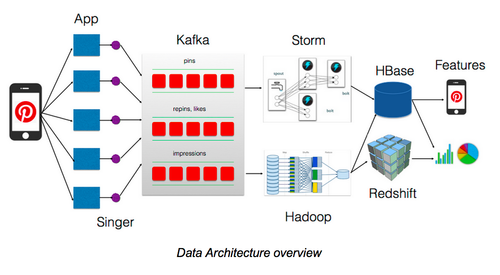
\includegraphics[width=1\textwidth]{pinterest_architecture.png}
	\caption{Schema - Architecture pinterest.com}
	\label{schema_pinterest_architecture}
\end{figure}
If you take a look at Figure \ref{schema_pinterest_architecture}, you can see a comparable data system architecture, implemented by pinterest.com\footnote{\cite{PINA}, Architecture of Giants: Data Stacks at Facebook, Netflix, Airbnb, and Pinterest}. Redis as a database on top of the hadoop cluster storage to serve for analytical purposes (e.g. ad serving of pinterest's adbuyers) or HBase on top of Hadoop cluster storage and Storm to serve features for the actual end-user of pinterest.com.\\

But we need to take care here: by creating new and more complex data systems from special purpose data systems, complexity is growing with it. How to ensure the system is avalaible with a reliable performance if something crashes? How to make sure data remains consistent and complete if things go wrong? How to scale the data system to be able to handle increased load?...\\
There are many apects which are crucial and influence the architecture of a data system like regulary constraints like data security, location of servers, SLA's\footnote{\cite{WKSLA}, \textit{Service Level Agreement, a commitment between a service provider and a client. Particular aspects of the service – quality, availability, responsibilities – are agreed between the service provider and the service user.}}\abk{SLA}{Service Level Agreement} or existing devlopment and operation skills - which very much depend on the specific situation.\\
Within the next chapters we will focus on the aspects which must be taken into account by any data system:

\begin{itemize}
			\item \nameref{tf_nfreq_scalability} (Chapter \ref{tf_nfreq_scalability}),
			\item \nameref{tf_nfreq_avrel} (Chapter \ref{tf_nfreq_avrel}),
			\item \nameref{tf_nfreq_maintainability} (Chapter \ref{tf_nfreq_maintainability}).\\
\end{itemize}

As many people and companies usually mess around with those terms, firstly we will develop a clear understanding on what they mean and later on take a closer look on how to apply algorithms, development and architectures to fulfill them appropriately.

\subsection{Scalability}
\label{tf_nfreq_scalability}
As is evident from the introduction of this chapter: the fact that a system is working reliable today doesn't mean it will necessarily work reliable in the future. The data system of ebay.com in 1999 was maxed out at handling \textbf{50.000} active listings\footnote{\cite{EBAYA}, slide 9}, imagine how the system would behave today at handling \textbf{1 billion} active listings\footnote{\cite{EBAYHP}}.
Obviously handling increased load (e.g. a larger amount of data needed to store or request to handle) is a major factor of a scalable data system.
\\[0.5 cm]
\hspace*{4mm}%
\fbox{%
  \hspace*{1.5mm}\hspace*{-1\fboxsep}%
  \parbox{0.08\textwidth + 5mm - 2\fboxsep}{%
\begin{minipage}{0.1\textwidth}

\includegraphics[width=\linewidth]{gear_brain.png}
\end{minipage}
  }%
}\hspace*{4mm}%
\begin{minipage}{0.8\textwidth}\raggedright
\textbf{Scalability} is the capability of data system to handle a growing amount of load (e.g. a larger amount of data needed to store or requests to handle). A data system is considered scalable if its capable of increasing it's total through-/output under an increased load when resources (typically hardware) are added. \\
\end{minipage}\\[0.4 cm]

Note that, ``\textit{scalability}'' isn't a binary tag that could be attached to a data system. It's pointless to say ``\textit{a data system is scalable}'' as well as ``\textit{a data system is not scalable}'', in either way you must think about ``\textit{If the load of a data system grows in a certain way, what are the options on the table for coping with the growth?}'' and ``\textit{How can we add ressources (hardware) to be able to handle the additional load?}''. \\
Therefore we will discuss the parameters and definition of \textbf{Load} (Section \ref{tf_nfreq_scalability_load}) and \textbf{Performance} (Section \ref{tf_nfreq_scalability_performance}) within the next section as well as \textbf{Approaches} for coping with load to achieve a certain performance (Section \ref{tf_nfreq_scalability_approaches}).

\subsubsection{Load}
\label{tf_nfreq_scalability_load}
To get an idea what \textit{load} of a data system actually means, how it could be described an measured, we will take a nother look at the example of ebay.com discussed so far. If we take a look back at the architecure of ebay at 1997-1999 (Figure \ref{schema_ebay_architecture_1997_1999} on page \pageref{schema_ebay_architecture_1997_1999}) we can already guess with increasing load (page requests to certain items listed on ebay.com and in this way calls to the database through the application) will reach its limit at the maximum amount of read requests the oracle database can serve. As the application tier (web server) has already been scaled horizontally to multiple nodes, the oracle database server reached its limit of physical growth in November 1999. \\
\begin{figure}[ht]
	\centering
  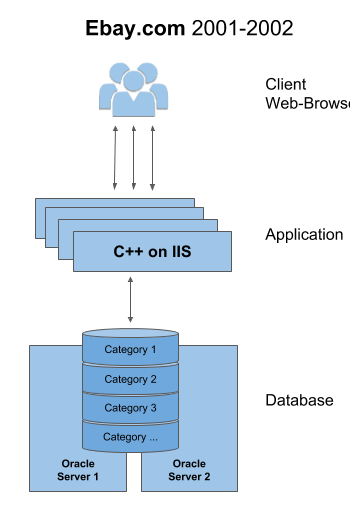
\includegraphics[width=0.4\textwidth]{Ebay_2002.png}
	\caption{Schema - Architecture Ebay.com April 2001 - December 2002}
	\label{schema_ebay_2002}
\end{figure}


So ebay added an additional server to not just elmininate the SPOF\abk{SPOF}{Single Point Of Failure}\footnote{\cite{WPSPOF}, Single Point Of Failure} but to be able to failover but also they have splitted the database to be able to logically partition it into separate instances and in this way be able to scale horizontally. This was achieved in 2001 by splitting items by categories, as you can see in Figure \ref{schema_ebay_2002} on page \pageref{schema_ebay_2002}. In this simple way it was possible to distribute the load (mostly page requests for items) in an ``equal'' way to different physical nodes.
Later on they segmented whole databases into functional areas like hosts for item, user, account or transaction data as well as partitioned the data by typical usage characteristics to scale horizontally.\\

They obviously did furher optimizations at the whole data system to be able to cope with the increasing load, like disabling transactions, moving CPU-intensive\abk{CPU}{Central Processing Unit}\footnote{CPU, a processor or processing unit is an electronic circuit which performs operations on some external data source, usually memory or some other data stream is called central processing unit} work to the application tier (e.g. joins, referential integrity or sorting), extensive use of prepared statements...but as this techniques are not mainly specific for distributed systems and some of them not even recommened nowadays, we won't focuse on them within this lecture.\\

In the example of ebay.com, requests per item and category could be a valuable \textit{load parameter} for discussing scalability, since it determines the database requests per data record and partition - as proven by the the data system structure of ebay at 2002 as we see.
Your or other data systems you have seen so far most likely have very different characteristics, but you can apply similar principles to reason about their load.
\\[0.5 cm]
\hspace*{4mm}%
\fbox{%
  \hspace*{1.5mm}\hspace*{-1\fboxsep}%
  \parbox{0.08\textwidth + 5mm - 2\fboxsep}{%
\begin{minipage}{0.1\textwidth}

\includegraphics[width=\linewidth]{gear_brain.png}
\end{minipage}
  }%
}\hspace*{4mm}%
\begin{minipage}{0.8\textwidth}\raggedright
The \textbf{load} of a data system is a measurement of the amount of computational work it performs (depending on the architecture in-place), e.g. the number of (concurrent) reads from a data storage, writes to a data storage or the ratio between reads and writes. The maximum load is defined by the weakest part of the architecture (=\textit{bottleneck}). \\[0.4 cm]
\end{minipage}\\

\subsubsection{Performance}
\label{tf_nfreq_scalability_performance}
Now that we have described what \textit{load} of a data system means as well as what \textit{load parameters} could be, we will examine more closely what happens when the load increases. Usually there are two important cases you need to think about while developing data systems:\\
\begin{samepage}
\begin{itemize}
			\item The load parameter increases, but all ressources (e.g. number of server, CPU or memory) stay the same - how is the performance of the data system affected?
			\item The load parameter increases - how much do you need to increase the ressources (e.g. number of server, CPU or memory) to keep the performance stay the same?\\
\end{itemize}
\end{samepage}

But how to answer them? Therefore we need performance numbers. In case of data systems measurement, methods usually are \textbf{throughput} (number of records that can be handled), e.g.:
\begin{itemize}
			\item read/writes per second (in case of MongoDB up to 100.000 read/writes per second)
			\item messages processed (in case of Apache Kafka and Linkedin more than 2 million records per second on just 3 nodes)
			\item data processed (in case of Apache Hadoop and MapReduce terabytes of data within several seconds)\\
\end{itemize}

or if your buidling a data-system which works as the backend of a end-user facing application like a website, it's more about the \textbf{response time}, which means the time between sending a request and receiving the response. For instance if we think about the example of ebay.com within the previous chapters, as of 2012 they had 1 billion items accessible at any time, needed to serve 2 billion page requests each day and had to fulfill each of them within fractions of a second\footnote{\cite{EBAY2012}, https://hughewilliams.com/2012/06/26/the-size-scale-and-numbers-of-ebay-com/}. \\

Regardless of throughput or response time - if we think about performance we don't think about a single number, but a distribution of values that we can measure. If you will repeat the same page request, read or writes on the same data system: response time and throughput will inevitable vary somehow. There are simply too many factors you usually cannnot contain:
\begin{itemize}
			\item network issues (e.g. latency or TCP packet loss and retransmission)
			\item os issues (e.g. a page faults, context switches or running background processes)
			\item physical issues (e.g. a damaged disk/ssd or overheating of a CPU and, associated therwith a decreased processing power) \\
\end{itemize}

Therfore it is common to use an average for measuring throughput or response times. \textit{Average} doesn't refer to a particular formula, we will briefly discuss 3 that are commonly used:
\begin{itemize}
			\item \textbf{arithmetic mean}\footnote{Sum of values divided by the number of values.} (easy to calculate but ignores ratios and is highly affected by statistical outliers, so it cannot tell you how many requests, reador writes actually have had a worse performance)
			\item \textbf{median}\footnote{A median separates the higher half of values from the lower half.} (easy to calculate and less distorted by outliers)
			\item \textbf{percentiles}\footnote{A measure used for indicating a certain percentage of scores falls below that measure.} (easy to calculate, not distorted by outliers) \\
\end{itemize}

\begin{figure}[ht]
	\centering
  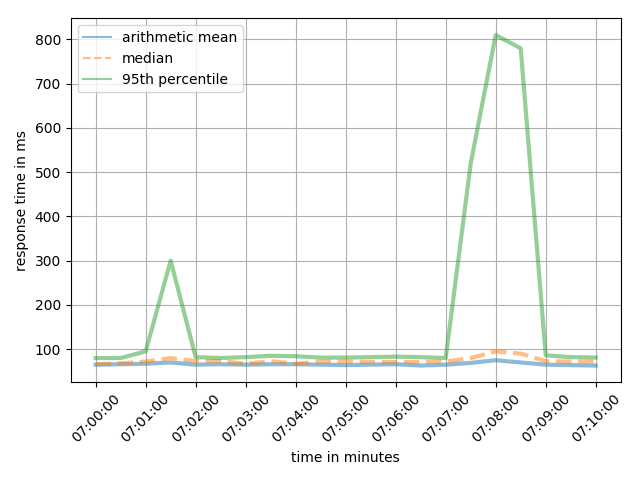
\includegraphics[width=1\textwidth]{mean_average_percentile_plot.png}
	\caption{Schema - Arithmetic Mean, Median and Percentiles Example}
	\label{schema_mean_average_percentile_plot}
\end{figure}

As you can guess, evaluating symmetric distributions with no outliers, \textit{arithmetic mean} will be the best choice, but as we are looking at performance parameters like throughput and response times, symmetric distribution is a whishful thinking. More usually throughput and response times will result in skewed distributions, so \textit{median} seems to be the better choice, as it doesn't ignore ratio and outliers completely. For instance if you calculate the median for latency (y-axis) of reads in a given timeframe (x-axis) from a data system as illustrated in figure \ref{schema_mean_average_percentile_plot} on page \pageref{schema_mean_average_percentile_plot}. You can see a small peak at \textit{07:08:00} but it still looks fine as the median response time is < 100ms. But what about the green graph (\textit{95th percentile})? That's the main reason why using percentiles is pretty common, especially the 95th, 99th or 99.9th percentile (abbreviated \textit{p95}, \textit{p99}, \textit{p999}) is frequently used in SLA's\footnote{\cite{WKSLA}, \textit{Service Level Agreement, a commitment between a service provider and a client.}}. Percentiles define thresholds at which 95\%, 99\% or 99,9\% of requests, reads or writes are beneath that threshold. Looking back at figure \ref{schema_mean_average_percentile_plot} this would mean that 95\% of all requests, reads or writes done by user are faster or equal 810ms and 5\% will result in a response time > 810 ms, which in case of a customer facing data system could mean: 5\% unsatisfied users and in this way probably a loss of possible leads (e.g. purchases on a webshop or subscriptions for a video streaming platform) and ultimately loss of revenue.\\
So why don't use 99,9th percentile every time as it is the best? This is a major cost factor, optimizing the last percentiles gets really expensive, especially as this usually involves a lot of hardware redundancy as well as eliminating factors outside of your control. At a certain point costs will be bigger than the benefits, so you need to make a trade-off. \\[0.5 cm]
\hspace*{4mm}%
\fbox{%
  \hspace*{1.5mm}\hspace*{-1\fboxsep}%
  \parbox{0.08\textwidth + 5mm - 2\fboxsep}{%
\begin{minipage}{0.1\textwidth}

\includegraphics[width=\linewidth]{gear_brain.png}
\end{minipage}
  }%
}\hspace*{4mm}%
\begin{minipage}{0.8\textwidth}\raggedright
\textbf{Performance} of a data system is defined by system throughput and response time, e.g. number of transactions (like read/write operations), processed records (like aggregations for analytical purposes) or even system commands (like an \textit{update statistics} or rebalancing of several data nodes) under a given workload and for a specific timeframe. It usually depends on a variety of influencable as well as uninfluencable factors of the system itself, like network latency, a page fault or damaged disk. \\[0.4 cm]
\end{minipage}\\

\subsubsection{Approaches For Scaling}
\label{tf_nfreq_scalability_approaches}
Now that we are familiar with describing \textit{load} and measuring \textit{perfromance} we can answer the question: how to ensure performance, even if the load increases?
As we have seen by the example of ebay.com within the previous chapters, a system which is able to cope with a load, won't be able to handle 10 times of that load. This needs us to think about the architecture right at the beginning as well as each time the load significantly increases. As we have learned there are two ways to scale an architecture of a data-system:

\begin{itemize}
			\item \textbf{scale up/vertical} - replace a server by a more powerful one
			\item \textbf{scale out/horizontal} - distribute the load towards multiple server instead of one\\
\end{itemize}

A data-system running on a single server is easier to develop, as you can neglect a lot of factors that are specific to distributed systems (e.g. replication, partitioning or transactions and consistency across nodes), but more powerful machines are also more expensive and at a certain point you will reach the physical limit as ebay.com did. \\
A distributed data-system will require more development, test and operational effort as well as result in complexity but servers will be much cheaper as you make use of less powerful machines (\textit{``commodity'' hardware}) and you are able to bypass the inevitable physical limit of a single server. \\
In practise you won't choose one pattern only (scale up or out) as well-working architectures need a carefully chosen mixture of both approaches, e.g. it doesn't make sense to make use of a lot of poorly powered servers (like a Raspberry Pi) instead of some more powerful machines in terms of unnecessary costs, network and software complexity. As you may guess, there is no one-size-fits-all solution and architecture for scalabale data-systems as the requirements are highly specific to each data-system itself. The \textit{load parameter} may be strongly influenced by:

\begin{itemize}
			\item the \textbf{volume of data} to store
			\item the \textbf{number of read or write operations}
			\item the required \textbf{throughput} or \textbf{response time}
			\item the \textbf{structure of the data} and \textbf{how it's accessed} (e.g. relational, document-oriented, graph)
			\item and many more.\\
\end{itemize}

Right now it shall be sufficient that you know the basics concepts of scalability, later within this lecture, we will make use of it when looking at distributed data storage and processing as well as related software and frameworks. At the end you should be able to apply those concepts to any data-system and be able to make reasonable decisions in terms of scalability.

\newpage

\subsection{Reliability}
\label{tf_nfreq_avrel}
In general \textit{reliability} represents the probability that something/someone will perform a required function without failure under stated conditions for a period of time, e.g. a test will be reliable when it gives the same repeated result under the same conditions. \\Or more pragmatic: \textit{something works correctly even if things go wrong}.\\

So what are the \textit{faults}, mentioned in the previous defintions that we need to anticipate, about?

\subsubsection{Hardware Faults}
\label{tf_nfreq_reliability_hardware_faults}

Obviously any hardware produced has a certain lifespan, buth that's not the only reason for hardware faults. If you're talking with operators of data centers, they will provide you with a broad list of common as well ase spine-chilling causes for hardware faults as:\\

\begin{itemize}
			\item broken HDDs\abk{HDD}{Hard Disk Drive}\footnote{HDD, a hard disk drive is a non-volatile computer storage device containing magnetic disks or platters rotating at high speeds.} or SSDs\abk{SSD}{Solid-State Drive}\footnote{SSD, a solid-state drive is a nonvolatile storage device that stores persistent data on solid-state flash memory.}
			\item faulty RAM\abk{RAM}{Random Access Memory}\footnote{RAM, a Random Access Memory is the hardware in a computing device where the operating system, application programs and data in current use are kept so they can be quickly reached by the device's processor.} or CPUs\footnote{CPU, a processor or processing unit is an electronic circuit which performs operations on some external data source, usually memory or some other data stream is called central processing unit}
			\item broken power adapters, switches or whole network outages
			\item unplugged network cables or even connected to the wrong port
			\item and many many more.\\
\end{itemize}

As this seems pretty unlikely at first sight - it's definitely not. For instance let's have a look at hard drives, especially in distributed data-systems you will have a lot of them. If you think about Apache Hadoop, you usually use low-class server (\textit{``commodity'' hardware}), e.g. \textit{ProLiant DL380 Gen10 Server} as they provide a good ratio of:

\begin{itemize}
			\item computing power (CPU) / Storage (HDD), 
			\item rack space (2 RU\abk{RU}{Rack Unit}\footnote{\cite{WPRU}, Rack Unit is a unit of measure defined as 44.50 millimetres (1.75 in). It is most frequently used as a measurement of the overall height of rack frames.}) / storage and 
			\item benefit/cost.\\
\end{itemize}
Each of this servers can store 19 HDDs, if you build a hadoop cluster with those servers, e.g. with about 100 nodes, this means 1,900 HDDs. Based on a regularly study by BackBlaze\footnote{\cite{HDDSTDY}, https://www.backblaze.com/blog/hard-drive-failure-rates-q1-2017/} (a big data storage center provider like Amazon AWS) with a set of 82,516 HDDs, the average annual failure rate is about 2.11\%. Regarding our previous Hadoop example containing 1.900 HDDs, we can suppose that nearly any week a HDD will fail. If we would make use of the particular HDD model \textit{Seagate ST4000DX00} with a failure rate of 35,88\% (also mentioned within the study) this would mean nearly 2 HDDs would fail each day.\\

In single server data systems it is possible to mitigate those problems by adding redundancy to individual hardware parts to minimize the failure rate of the whole system to a point where a failure is very unlikely, as at any time a redundant part can take over. This could mean, dual power adapters (like used by the previous mentioned \textit{ProLiant DL380 Gen10 Server}), RAID\abk{RAID}{Redundant Array of Independent Disks}\footnote{RAID, is a data storage virtualization technology that combines multiple physical disk drive components into one or more logical units for the purposes of data redundancy, performance improvement, or both.} configurations or hot-swappable CPUs.
As data volumes and computing demand increases, data-systems need to be distributed among several servers, which proportionally increases the rate of hardware faults and system failures, like discussed above regarding HDD faults. Therefore distributed data systems need to be able to tolerate the loss of entire machines, requiring software to be fault-tolerance additionally to hardware redundancy. 
But those distributed data systems have further advantages, a system that tolerates failure of single machines can be restarted, patched, updated (\textit{rolling-upgrades}) or maintained - one node at a time - without a downtime of the whole data-system.

\subsubsection{Software Faults}
\label{tf_nfreq_reliability_software_faults}
When we talk about software faults in terms of distributed data-systems, we don't talk about usual bugs but rather faults which affect the whole data-system integrity and reliability. Such faults are harder to anticipate than usual bugs of single-server applications, as they usually tend to be caused by the environment (e.g. multiple servers, network, dependencies, special and unusual circumstances), are difficult to test, and are even worse in their result as they can cause a failure of the whole data-system.
Examples could be:
\begin{itemize}
			\item a runaway and/or zombie process that extensively used up some shared ressource (e.g. network, CPU, RAM, disk space)
			\item a software bug causing the whole cluster to fail (e.g. the Hadoop Ressource Manager YARN\abk{YARN}{Yet Another Resource Negotiator}\footnote{YARN, Yet Another Resource Negotiator} once had a bug\footnote{\cite{YARNKPBUG}, https://issues.apache.org/jira/browse/YARN-2809}, that if you removed a cgroup (\textit{control group}) under some circumstances (\textit{race conditions}) a kernel panic and in this way a failure of multiple server was caused
			\item a service the whole data-system depends on slows done, becomes unresponsive or fails
			\item cascading failures (e.g. one server of the data-system fails due to heavy network traffic, causing the other servers to take over, in this way increasing network traffic for them too and finally all server will fail)\\
\end{itemize}

As you can see, most of the reasons for software faults are caused by assumptions about the environment that may not be true at some time and at some special circumstances. To avoid suffering those issues you need to carefully think about assumptions and interactions within the distributed data-system, you will need a lot of measuring, monitoring and you will do a lot of analyzing of the system behaviour in any special circumstance as well as testing even with forcing some servers of the system to crash.

\subsubsection{Human Faults}
\label{tf_nfreq_reliability_human_faults}

We have been talking a lot about reliability so far, but what about the most unreliable factor: humans. We will briefly discuss some approaches to make a data-system reliable in terms of unreliable humans:
\begin{itemize}
			\item decouple places where people make the most failures from places they can cause failures, e.g. using production and development environments or providing interfaces or frameworks for an API instead of direct API access
			\item use extensive testing (e.g. unit test, system tests, integration tests) and automize them
			\item measuring and monitoring (e.g. performance metrics, error rates) allows to check wether assumptions or constraints are violated at an early stage \\[0.5 cm]
\end{itemize}

To sum up the last chapters: why do wee need reliability? Reliability is not just a major topic for stock exchanges, air line reservations or military. Failures of a data-system can cause data loss, lost productivity or sales loss and therefore huge costs and loss of revenue. There are special circumstances when you may choose to reduce reliability for the sake of time, development effort or operational costs (e.g. \textit{prototyping}), but you need to be very conscious and it's inevitable that at some point in the future you will need to invest the the saved effort, time and costs and probably a multiple of what it would have been before.\\[1.0 cm]
\hspace*{4mm}%
\fbox{%
  \hspace*{1.5mm}\hspace*{-1\fboxsep}%
  \parbox{0.08\textwidth + 5mm - 2\fboxsep}{%
\begin{minipage}{0.1\textwidth}

\includegraphics[width=\linewidth]{gear_brain.png}
\end{minipage}
  }%
}\hspace*{4mm}%
\begin{minipage}{0.8\textwidth}\raggedright
\textbf{Reliability} in terms of hardware, software or especially data-systems can be defined as the ability of a system to function as specified and expected. A reliable data-system also detects and tolerates faults due to mistakes of users, hardware or lower parts of the data-system itself as well as ensures the required performance under any expected load. \\[0.4 cm]
\end{minipage}\\

\subsection{Maintainability}
\label{tf_nfreq_maintainability}
Maintenance is known as one of the biggest costs at software devlopment and in the same way a very unfamous topic to software engineers. Keeping a system running, investigating failures, fixing bugs, adding new features, adapting it to updates of underlying hard- and software - to name some usual tasks.\\

A data-system should be designe to minimize effort during maintenance and in this way making it more reliable. We will briefly discuss 3 major topics: \textit{operability}, \textit{simplicity} and \textit{evolvability}.

\subsubsection{Operability}
\label{tf_nfreq_maintainability_operability}
The main goal of operability should be to make operations easy to keep the system running smoothly, this means making routine tasks easy and enable operations ressources to use their time for important tasks. This can be achieved by:
\begin{itemize}
			\item good documentation and operational model (a data-system which can be understand easily can be operated more easily)
			\item transparency (visibility into the data system and runtime behaviour, e.g. by log files or monitoring tools)
			\item no dependencies between single services or server (allow single server to go down for maintenance tasks, e.g. patches, update or restarts)
			\item self-healing if possible, but also possibilities to override for operators\\[0.5 cm]
\end{itemize}

\subsubsection{Simplicity}
\label{tf_nfreq_maintainability_simplicity}
When you start a development project everything is pretty simple and probably well-documented but later on with multiple developers, features, services and servers, it gets more complex, hard to understand by a developer and especially more difficult to handle by administrators. As a lot of issues caused by this are not specific to data-systems we will focuse on complexity and abstraction, as reducing complexity should be the main goal when devloping distributed data-systems. Making a system less complex doesn't require reducing functionaility, it's more about removing unnecessary complexity.\\
For instance if your data-system is crunching a lot of data for a very plain purpose, like parsing web server log files for analytical purpose to get to know how many people have visited your website - you could do this counting in Java (MapReduce) but this will probably be about 50 lines of code, a lot of libraries, testing and dependencies - making operations more difficult in the same way. If you would do this using Hive on HDFS your done with a one-line SQL statement.\\

However finding useful abstractions is not that easy and needs a lot of experience, but when you are developing something you should always ask yourself: do I make use of abstraction and will the complexity be at a manageable level?


\newpage
\section{Storage Concepts}
\label{tf_storageconcepts}
Lorem ipsum dolor sit amet, consetetur sadipscing elitr, sed diam nonumy eirmod tempor invidunt ut labore et dolore magna aliquyam erat, sed diam voluptua. At vero eos et accusam et justo duo dolores et ea rebum. Stet clita kasd gubergren, no sea takimata sanctus est Lorem ipsum dolor sit amet. Lorem ipsum dolor sit amet, consetetur sadipscing elitr, sed diam nonumy eirmod tempor invidunt ut labore et dolore magna aliquyam erat, sed diam voluptua. At vero eos et accusam et justo duo dolores et ea rebum. Stet clita kasd gubergren, no sea takimata sanctus est Lorem ipsum dolor sit amet.

\newpage

\section{Data Models And Access}
\label{tf_dma}
Data Models are one of the most crucial part of any data-system as they significantly influence actually everything: development and required skills, operations, backends and frontends as well. \\
For instance, if you choose a document oriented data store (e.g. MongoDB) to serve a web-based application, as it is pretty easy to build a REST API on top of it and JSON data and JavaScript Frontends (e.g. based on AngularJS) are a perfect match but don't think about how the data will be queried later - you may run into a lot of trouble. For example if your data consist of many business objects which are highly complementary and the frontend usually needs multiple business objects within one request, you're probably out of luck as document-oriented storages perform pretty well when only reading from one collection but not at joining them. You could probably put all related business objects in one document, but as this is unnecesessarily redundant it will burst your data storage very soon. \\
To conclude: there are many different kinds of data models and every data model has it strengths but weaknesses as well. Some are easy to use - some not, some operations using them will be fast - others definitely not, some are very storage efficient - some note... As you can see it's not that easy to decide which data model to use as it has a profound effects on the whole data-system you are building, even that far that a wrong decision could be a show stopper at some time in development.\\
It needs a lot of experience and very forward-looking to choose a data model that fits best to your data-system. Within the next chapters we will talk about the most common data models (\textit{relational}, \textit{document-oriented}, \textit{graph}), how to access them {\textit{SQL}, \textit{MapReduce}, \textit{SPARQL}), how they differ, advantages and disadvantages. \\
At the end you should have a basic understanding on how they work and which of them fits best to a certain problem.

\subsection{Data Models}
\label{tf_dma_datamodels}

\subsubsection{Relational Data Model}
\label{tf_dma_datamodels_rdm}

Firstoff we will take a look at the relational data model, originally introduced by Edgar Frank Codd in 1970\footnote{\cite{CODDRDM}, `A Relational Model of Data for Large Shared Data Banks'' - IBM Research Laboratory, San Jose, California}. \\[0.5 cm]
\hspace*{4mm}%
\fbox{%
  \hspace*{1.5mm}\hspace*{-1\fboxsep}%
  \parbox{0.08\textwidth + 5mm - 2\fboxsep}{%
\begin{minipage}{0.1\textwidth}

\includegraphics[width=\linewidth]{gear_brain.png}
\end{minipage}
  }%
}\hspace*{4mm}%
\begin{minipage}{0.8\textwidth}\raggedright
The \textbf{relational model} is an approach to managing data using a structure and language consistent with first-order predicate logic where all data is represented in terms of tuples and grouped into relations. 
\end{minipage}\\[0.5 cm]

Having its roots in the 1970's the relational data model had the idea to hide implementation details (e.g. internal representation of data in a data store) from developers by providing a cleaner, \textit{declarative} and \textit{read-on-schema} interface for specifying data and querying it. Developers can state what information the database contains and what information they want from it - the database itself will take care of describing, storing and retrieving data for developers. As you have already learned the basic about relational databases, indices, concepts like normalization and much more we will take a quick look at an example and afterwards conclude about advantages and disadvantages compared to other data models. \\

Let's take a look at figure \ref{schema_facebook_relational_model} on page \pageref{schema_facebook_relational_model} as an example. Here you can see how a Facebook profile could be represented in a very simple (and not fully normalized) relational data model. 
The table \lstinline{user} works as the main entity, as it's the profile page of a user. As a user is unique we also have a unique identifier (\lstinline{id}) as well as some information regarding the user within the same table (e.g. \lstinline{first} and \lstinline{last_name} or who they are \lstinline{married_to}). 
People may have worked for different companies (table \lstinline{companies}), lived in several cities {table \lstinline{cities}} or visited more than one university (table \lstinline{universities}) so we put that into separate tables including a foreign key (\lstinline{user_id}) of the referring table {\lstinline{user}}.\\

\begin{figure}[ht]
	\centering
  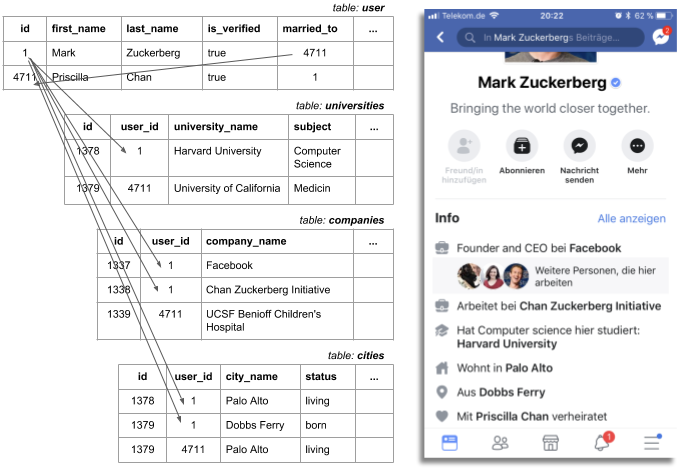
\includegraphics[width=1\textwidth]{relational_model_zuckerberg.png}
	\caption{Schema - Facebook Profile As Relational Model}
	\label{schema_facebook_relational_model}
\end{figure}

\newpage

Relations are represented by \textit{tables} and tuples are represented by \textit{rows}. Rows can easily be inserted or fetched all-at-once, by using an id or a \textit{primary}/\textit{foreign key} unlike \textit{document-oriented} data models, where you:
\begin{itemize}
			\item sometimes need to make use of access paths,
			\item need to think about nested structures,
			\item need to worry about unknown fields as those systems are usually \textit{schema-on-read} or 
			\item or intensively need to think about possible performance issues and how the system will probably execute your query as the execution engine is usually not that mature as the one of a relational system,
			\item it's more difficult to understand how the systems works, as sometimes you don't even have a query-explain feature like in relational databases, so you won't be able to investigate or guess in advance how it will behave in detail during execution.\\ 
\end{itemize}
But as relational data models are also mostly used by applications, we need to talk about a frequently discussed issue: \textit{object-orientation}. As applications are \textit{object-oriented} you need to make use of a translation layer between an applications and relational model to enable the applications to make use of the data. There are many frameworks available to serve this translation called ORM\abk{ORM}{Object-Relational-Mapper}\footnote{ORM, Object-relational mapping is a programming technique for converting data between incompatible type systems using object-oriented programming languages.}, e.g. Hibernate\footnote{\cite{ORMHBN}, http://hibernate.org/} in case of Java or SQLAlchemy\footnote{\cite{ORMSQLAL}, https://www.sqlalchemy.org/} in case of Python to name only 2 of them. Those frameworks will require additional code, skill and development time, as systems using the document-oriented model are regularly used without additional frameworks for data translation, e.g. an AngularJS application using MongoDB. \\
But systems using a relational model are mostly more resilient as they usually gained several years or even decades of research, experience and development time, while document-oriented that are still widely used today just started in the early 2000's.\\
For instance many of them have highly sophisticated query optimizer which automatically decide which part of the query needs to be executed when, in which order and which index {e.g. \lstinline{user_id} of the previous example} is probably the best one to use - most of the document-oriented systems don't even have something that is worth to be called a query optimizer as their capabilities are far behind the relational ones. \\
But that's also due to the fact that relational and document-oriented data models are completely different in terms of relationship implementation: both of them are able to represent \textit{many-to-one} or \textit{many-to-many} relations but in a different manner. \\
Relational data models make use of \textit{primary} and \textit{foreign keys} which can easily be used for indices, document-oriented data models need to make use of nested structures (most commonly used) or \textit{document references} and joins to other collections (e.g. \lstinline{\$lookup} in MongoDB\footnote{\cite{MDBLKP}, https://docs.mongodb.com/manual/reference/operator/aggregation/lookup/}, \lstinline{populate()} in Mongoose\footnote{\cite{MGPPL}, http://mongoosejs.com/docs/populate.html} or Joins in RethinkDB\footnote{\cite{RDBJN}, https://www.rethinkdb.com/docs/table-joins/}) - both of them are resulting in expensive IO and CPU operations as either you need to make use of features that are extremely immature compared to their relational counterpart or the whole document needs to be read, which can also be very wasteful on large documents. \

This behaviour of document-oriented systems also applie for writes, as they usually require to rewrite the whole document in document-oriented data-systems. 
But to be fair, most document-oriented systems weren't initially designed with serving relationale dependencies or querying in mind, but rather for the sake and benefits of: 
\begin{samepage}
\begin{itemize}
		\item being object oriented, 
		\item easy to be altered, 
		\item  being semi-/unstructured and schema-``free''.\\
\end{itemize}
\end{samepage}
An in this way being the whole opposite of the relational data model.


\subsubsection{Document Oriented Data Model}
\label{tf_dma_datamodels_dodm}

Text...

\begin{figure}[ht]
	\centering
  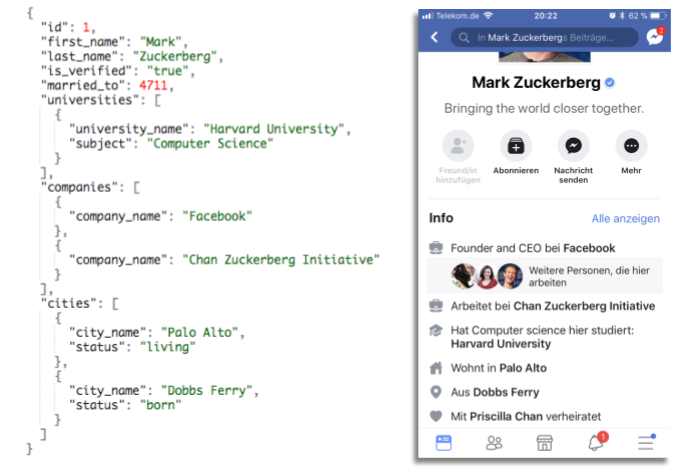
\includegraphics[width=1\textwidth]{document_oriented_data_model_zuckerberg.png}
	\caption{Schema - Facebook Profile As Document Oriented Model}
	\label{schema_facebook_document_oriented_model}
\end{figure}


\subsubsection{Graph Data Model}
\label{tf_dma_datamodels_gdm}

\subsection{Data Access}
\label{tf_dma_dataaccess}

\subsubsection{SQL}
\label{tf_dma_dataaccess_sql}

\subsubsection{MapReduce}
\label{tf_dma_dataaccess_mr}

\subsubsection{SPARQL}
\label{tf_dma_dataaccess_sparql}

\section{Challenges Of Distributed Data Systems}
\label{tf_dds}
Lorem ipsum dolor sit amet, consetetur sadipscing elitr, sed diam nonumy eirmod tempor invidunt ut labore et dolore magna aliquyam erat, sed diam voluptua. At vero eos et accusam et justo duo dolores et ea rebum. Stet clita kasd gubergren, no sea takimata sanctus est Lorem ipsum dolor sit amet. Lorem ipsum dolor sit amet, consetetur sadipscing elitr, sed diam nonumy eirmod tempor invidunt ut labore et dolore magna aliquyam erat, sed diam voluptua. At vero eos et accusam et justo duo dolores et ea rebum. Stet clita kasd gubergren, no sea takimata sanctus est Lorem ipsum dolor sit amet.

	\subsection{Partitioning}
	\label{tf_dds_partitioning}
	Lorem ipsum dolor sit amet, consetetur sadipscing elitr, sed diam nonumy eirmod tempor invidunt ut labore et dolore magna aliquyam erat, sed diam voluptua. At vero eos et accusam et justo duo dolores et ea rebum. Stet clita kasd gubergren, no sea takimata sanctus est Lorem ipsum dolor sit amet. Lorem ipsum dolor sit amet, consetetur sadipscing elitr, sed diam nonumy eirmod tempor invidunt ut labore et dolore magna aliquyam erat, sed diam voluptua. At vero eos et accusam et justo duo dolores et ea rebum. Stet clita kasd gubergren, no sea takimata sanctus est Lorem ipsum dolor sit amet.

	\subsection{Replication}
	\label{tf_dds_replication}
	Lorem ipsum dolor sit amet, consetetur sadipscing elitr, sed diam nonumy eirmod tempor invidunt ut labore et dolore magna aliquyam erat, sed diam voluptua. At vero eos et accusam et justo duo dolores et ea rebum. Stet clita kasd gubergren, no sea takimata sanctus est Lorem ipsum dolor sit amet. Lorem ipsum dolor sit amet, consetetur sadipscing elitr, sed diam nonumy eirmod tempor invidunt ut labore et dolore magna aliquyam erat, sed diam voluptua. At vero eos et accusam et justo duo dolores et ea rebum. Stet clita kasd gubergren, no sea takimata sanctus est Lorem ipsum dolor sit amet.

	\subsection{Transactions}
	\label{tf_dds_transactions}
	Lorem ipsum dolor sit amet, consetetur sadipscing elitr, sed diam nonumy eirmod tempor invidunt ut labore et dolore magna aliquyam erat, sed diam voluptua. At vero eos et accusam et justo duo dolores et ea rebum. Stet clita kasd gubergren, no sea takimata sanctus est Lorem ipsum dolor sit amet. Lorem ipsum dolor sit amet, consetetur sadipscing elitr, sed diam nonumy eirmod tempor invidunt ut labore et dolore magna aliquyam erat, sed diam voluptua. At vero eos et accusam et justo duo dolores et ea rebum. Stet clita kasd gubergren, no sea takimata sanctus est Lorem ipsum dolor sit amet.

	\subsection{Consistency}
	\label{tf_dds_consistency}
	Lorem ipsum dolor sit amet, consetetur sadipscing elitr, sed diam nonumy eirmod tempor invidunt ut labore et dolore magna aliquyam erat, sed diam voluptua. At vero eos et accusam et justo duo dolores et ea rebum. Stet clita kasd gubergren, no sea takimata sanctus est Lorem ipsum dolor sit amet. Lorem ipsum dolor sit amet, consetetur sadipscing elitr, sed diam nonumy eirmod tempor invidunt ut labore et dolore magna aliquyam erat, sed diam voluptua. At vero eos et accusam et justo duo dolores et ea rebum. Stet clita kasd gubergren, no sea takimata sanctus est Lorem ipsum dolor sit amet.
\chapter{Data Processing On Distributed Systems}
\label{chapter_data_processing}
\setlength{\epigraphwidth}{0.8\textwidth}
\setlength\epigraphrule{0pt}
\epigraph{\itshape Begin at the beginning, the King said gravely, ``and go on till you come to the end: then stop.''}{---Lewis Carroll, \textit{Alice in Wonderland}}

\section{Batch Processing}
\label{dp_batch}
to-be-added

\section{Micro-Batch Processing}
\label{dp_mb}
to-be-added

\section{Stream Processing}
\label{dp_stream}
to-be-added

\section{Message Queuing}
\label{dp_mq}
to-be-added


\section{ETL and Workflow Automation}
\label{dp_etl_wfl}
to-be-added
\chapter{Software and Frameworks}
\label{chapter_software_frameworks}
\setlength{\epigraphwidth}{0.8\textwidth}
\setlength\epigraphrule{0pt}
\epigraph{\itshape Begin at the beginning, the King said gravely, ``and go on till you come to the end: then stop.''}{---Lewis Carroll, \textit{Alice in Wonderland}}

to-be-added
\chapter{Data Science}
\label{chapter_data_science}
\setlength{\epigraphwidth}{0.5\textwidth}
\setlength\epigraphrule{0pt}
\epigraph{\itshape ``Big data is not bout the data.''}{--- Gary King, \textit{Harvard University}}

\section{Data Cleaning, Integration and Preparation}
\label{ds_}
Lorem ipsum dolor sit amet, consetetur sadipscing elitr, sed diam nonumy eirmod tempor invidunt ut labore et dolore magna aliquyam erat, sed diam voluptua. At vero eos et accusam et justo duo dolores et ea rebum. Stet clita kasd gubergren, no sea takimata sanctus est Lorem ipsum dolor sit amet. Lorem ipsum dolor sit amet, consetetur sadipscing elitr, sed diam nonumy eirmod tempor invidunt ut labore et dolore magna aliquyam erat, sed diam voluptua. At vero eos et accusam et justo duo dolores et ea rebum. Stet clita kasd gubergren, no sea takimata sanctus est Lorem ipsum dolor sit amet.

\section{Data Visualization}
\label{dp_batch}
Lorem ipsum dolor sit amet, consetetur sadipscing elitr, sed diam nonumy eirmod tempor invidunt ut labore et dolore magna aliquyam erat, sed diam voluptua. At vero eos et accusam et justo duo dolores et ea rebum. Stet clita kasd gubergren, no sea takimata sanctus est Lorem ipsum dolor sit amet. Lorem ipsum dolor sit amet, consetetur sadipscing elitr, sed diam nonumy eirmod tempor invidunt ut labore et dolore magna aliquyam erat, sed diam voluptua. At vero eos et accusam et justo duo dolores et ea rebum. Stet clita kasd gubergren, no sea takimata sanctus est Lorem ipsum dolor sit amet.

\section{Regression}
\label{dp_batch}
Lorem ipsum dolor sit amet, consetetur sadipscing elitr, sed diam nonumy eirmod tempor invidunt ut labore et dolore magna aliquyam erat, sed diam voluptua. At vero eos et accusam et justo duo dolores et ea rebum. Stet clita kasd gubergren, no sea takimata sanctus est Lorem ipsum dolor sit amet. Lorem ipsum dolor sit amet, consetetur sadipscing elitr, sed diam nonumy eirmod tempor invidunt ut labore et dolore magna aliquyam erat, sed diam voluptua. At vero eos et accusam et justo duo dolores et ea rebum. Stet clita kasd gubergren, no sea takimata sanctus est Lorem ipsum dolor sit amet.

\section{Classification}
\label{dp_batch}
Lorem ipsum dolor sit amet, consetetur sadipscing elitr, sed diam nonumy eirmod tempor invidunt ut labore et dolore magna aliquyam erat, sed diam voluptua. At vero eos et accusam et justo duo dolores et ea rebum. Stet clita kasd gubergren, no sea takimata sanctus est Lorem ipsum dolor sit amet. Lorem ipsum dolor sit amet, consetetur sadipscing elitr, sed diam nonumy eirmod tempor invidunt ut labore et dolore magna aliquyam erat, sed diam voluptua. At vero eos et accusam et justo duo dolores et ea rebum. Stet clita kasd gubergren, no sea takimata sanctus est Lorem ipsum dolor sit amet.

\section{Clustering}
\label{dp_batch}
Lorem ipsum dolor sit amet, consetetur sadipscing elitr, sed diam nonumy eirmod tempor invidunt ut labore et dolore magna aliquyam erat, sed diam voluptua. At vero eos et accusam et justo duo dolores et ea rebum. Stet clita kasd gubergren, no sea takimata sanctus est Lorem ipsum dolor sit amet. Lorem ipsum dolor sit amet, consetetur sadipscing elitr, sed diam nonumy eirmod tempor invidunt ut labore et dolore magna aliquyam erat, sed diam voluptua. At vero eos et accusam et justo duo dolores et ea rebum. Stet clita kasd gubergren, no sea takimata sanctus est Lorem ipsum dolor sit amet.

\section{Association}
\label{dp_batch}
Lorem ipsum dolor sit amet, consetetur sadipscing elitr, sed diam nonumy eirmod tempor invidunt ut labore et dolore magna aliquyam erat, sed diam voluptua. At vero eos et accusam et justo duo dolores et ea rebum. Stet clita kasd gubergren, no sea takimata sanctus est Lorem ipsum dolor sit amet. Lorem ipsum dolor sit amet, consetetur sadipscing elitr, sed diam nonumy eirmod tempor invidunt ut labore et dolore magna aliquyam erat, sed diam voluptua. At vero eos et accusam et justo duo dolores et ea rebum. Stet clita kasd gubergren, no sea takimata sanctus est Lorem ipsum dolor sit amet.

\section{Neural Networks}
\label{dp_batch}
Lorem ipsum dolor sit amet, consetetur sadipscing elitr, sed diam nonumy eirmod tempor invidunt ut labore et dolore magna aliquyam erat, sed diam voluptua. At vero eos et accusam et justo duo dolores et ea rebum. Stet clita kasd gubergren, no sea takimata sanctus est Lorem ipsum dolor sit amet. Lorem ipsum dolor sit amet, consetetur sadipscing elitr, sed diam nonumy eirmod tempor invidunt ut labore et dolore magna aliquyam erat, sed diam voluptua. At vero eos et accusam et justo duo dolores et ea rebum. Stet clita kasd gubergren, no sea takimata sanctus est Lorem ipsum dolor sit amet.

\section{DataScience on Distributed Systems}
\label{dp_batch}
Spark ML
PySpark
\chapter{Outlook}
\label{outlook}
\setlength{\epigraphwidth}{0.8\textwidth}
\setlength\epigraphrule{0pt}
\epigraph{\itshape ``Big data is not bout the data.''}{--- Gary King, \textit{Harvard University}}


Lorem ipsum dolor sit amet, consetetur sadipscing elitr, sed diam nonumy eirmod tempor invidunt ut labore et dolore magna aliquyam erat, sed diam voluptua. At vero eos et accusam et justo duo dolores et ea rebum. Stet clita kasd gubergren, no sea takimata sanctus est Lorem ipsum dolor sit amet. Lorem ipsum dolor sit amet, consetetur sadipscing elitr, sed diam nonumy eirmod tempor invidunt ut labore et dolore magna aliquyam erat, sed diam voluptua. At vero eos et accusam et justo duo dolores et ea rebum. Stet clita kasd gubergren, no sea takimata sanctus est Lorem ipsum dolor sit amet.
%%%------------------------------------------------------------------------------%%%
%%% Ein Tätigkeitsschwerpunkt %%% 
%%%------------------------------------------------------------------------------%%%



\chapter{Appendix}
\label{Kapitel_Appendix}
		\newpage
		



\newpage 
\printnomenclature % Abkürzungsverzeichnis
\newpage 
\listoffigures % Grafikverzeichnis
\newpage
\lstlistoflistings
\newpage 
%\listoftables % Tabellenverzeichnis
%\newpage
\bibliographystyle{alphadin} % Literaturverzeichnis I
\bibliography{libr} 	  % Literaturverzeichnis II
\end{document}